% \begin{figure*}[ht!]
% \centering
%   \begin{subfigure}{0.3\textwidth}
%                 \centering
%     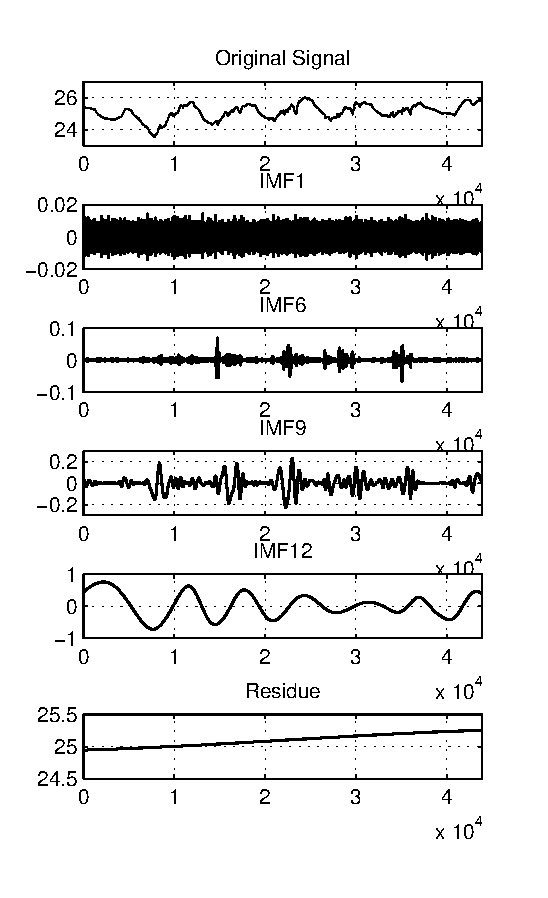
\includegraphics[width=\textwidth]{./fig/emd.eps}
%                 \caption{An example of EMD}
%                 \label{fig:emd}
%   \end{subfigure}
%   \begin{subfigure}{0.32\textwidth}
%                 \centering
%     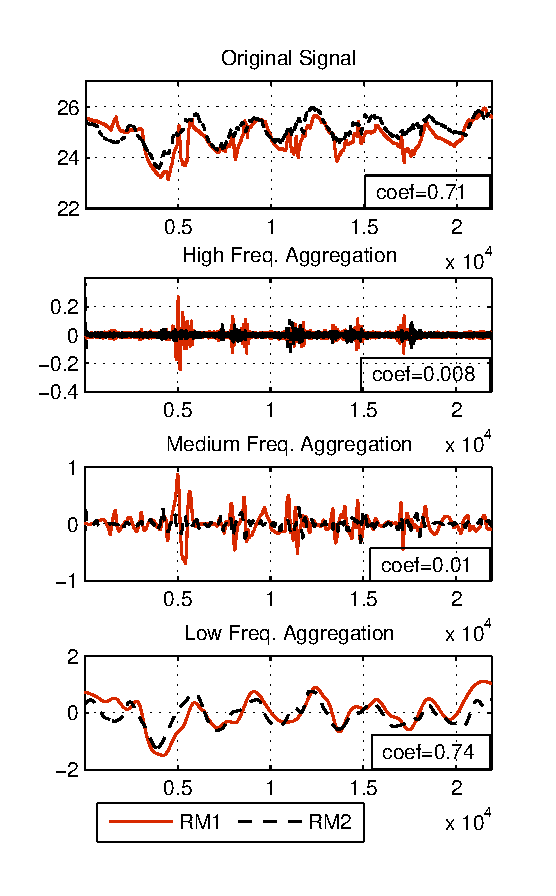
\includegraphics[width=\textwidth]{./fig/imf_aggr1.eps}
%                 \caption{IMFs aggregation}
%                 \label{fig:aggr1}
%   \end{subfigure}
%   \begin{subfigure}{0.32\textwidth}
%                 \centering
%     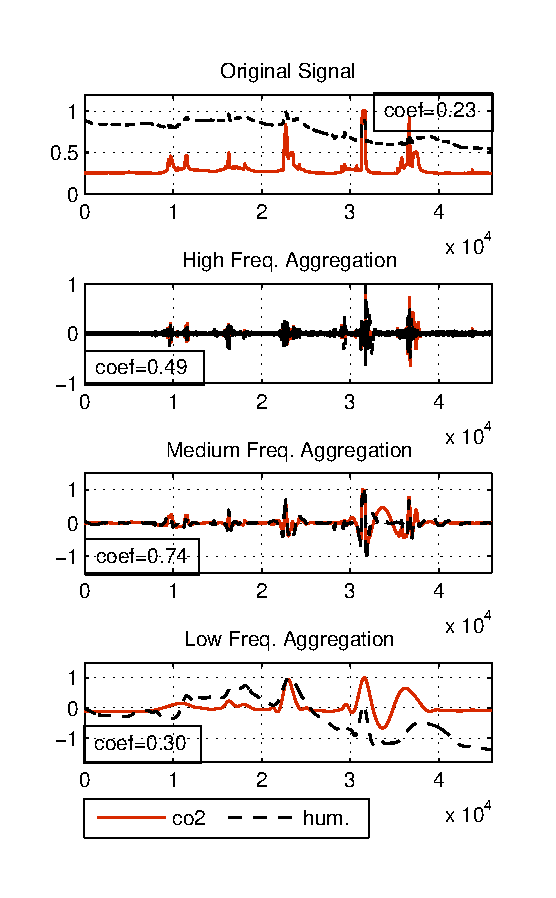
\includegraphics[width=\textwidth]{./fig/imf_aggr2.eps}
%                 \caption{IMFs aggregation}
%                 \label{fig:aggr2}
%   \end{subfigure}
% \caption{(a) EMD decomposes a signal and exposes intrinsic oscillatory components; (b) Aggregation of IMFs within a pre-defined frequency range makes seemingly similar signals from different locations more distinguishable; (c) IMF aggregation makes seemingly distinct signals of different sensors in the same room show high correlation.}
% \end{figure*}

\section{Methodology}
We first describe how we design the feature extraction and explain why the feature set works. Then we discuss
the classification technique we adopt as well as detail the training and testing process. In the end, we articulate
a solution to identifying potential misclassification when no ground truth labels for sensor types are available.

\subsection{Feature Extraction}
Raw sensor time series usually contain millions of readings which are too general to be informative for classification
tasks. We need to distill the information embedded in the sensor readings in the time domain. A signal in the time domain
trends the amplitude of a sensor reading and intuitively, different types of sensor would in general occupy distinct
amplitude bins as demonstrated in Figure~\cite{}. As to characterize the amplitude distribution of a signal in the time
domain, we can use percentiles in the readings, such as 25\%, 50\%, 75\% and so forth. Considering that there also
exist outlieres in sensor readings, we pick the 50\% (also known as the median number) for use as a discriminator, which
is more robust to outliers. However, on another side, sensor readings are subjective to the dynamics in the placed
surroudings therefore sensors of different types can collide in a same amplitude bin. For example, during a rainy season, the humidity in an
office can reach the range of 70~80 which is the same as typical temeprature sensor readings. Therefore, simply relying
on reading amplitude might not be able to effetively differentiate different sensors. Figure~\cite{} show some of such
examples. To capture these short term ``events'' as features, we also need to include the variance of the signals when
formulating a feature vector for the time series.

When extracting features from a raw sensor reading, the original trace can span over days, weeks or even months, and
the trends can vary a lot even from day to day. Therefore extracting the certain features such as percentiles and
variances from the entire sensor readings might make the features less discriminant, compared to doing so in shorter
windowed time slices. But computing features over windowed slices might end up producing too many elements for a
feature vector and also, having too many unnecessary feature variables might deteriorate the performance of classifier.
To better summarize the dynamics of sensor traces, we apply feature extraction to every X-minute long window and compute
the statistics of the accumulated features from windowed slices as the final features. 

As a summary, the feature extraction procedure goes as follows. First, each single sensor signal is segmented into N
non-overlapping X-minute long windows (we will discuss the decision of window length X in later section). Second, within
each time window, we compute the median and variance of the signal, obtaining a vector of medians and a vector of
variances after the window slides over the entire traces: 
\begin{displaymath}
\begin{split}
MED = \{median^{1}, median^{2}, ..., median^{N}\}\\
VAR = \{variance^{1}, variance^{2}, ..., variance^{N}\}
\end{split}
\end{displaymath}
Where N is the number of time windows. The vector $MED$ and $VAR$ reflect short term changes but not all the intermidiate values are essentially helpful for classification. So as a statistical summary of the two vectors, as a last step, for each vector we compute the minimun, maximun, median and variance, resulting in a feature vector of eight elements:
\begin{displaymath}
\begin{split}
F = \{min(MED), max(MED), median(MED), var(MED),\\
 min(VAR), max(VAR), median(VAR), var(VAR)\}
\end{split}
\end{displaymath}
And $F$ is the feature vector for each sensor trace used in our classification process.

\subsection{Classification}
After transforming all sensor time series into feature vectors, we leverage an ensemble classifier to achieve 
the type classification task. In general, ensemble learning methods obtain better predictive performance than
 any of the constituent learning methods~\cite{ensem1,ensem2}, if two assumptions hold~\cite{ensem3}: 1) the 
 probability of a correct classification by each individual classsifier is greater than 0.5 and 2) the errors
  in predictions of the base-level classifiers are independent. Random forests~\cite{RF} have been widely used 
  and outperform a single tree classifier. They are also faster~\cite{cvpr} in training and testing compared to traditional classifiers such as SVM. The notion of randomized trees was first introduced in~\cite{RT} and further well developed in~\cite{RF}.

Random forests grow a bunch of classification trees. To classify a new coming unlabeled object as a feature vector, 
feed the vector down each of the trees in the forest. Each tree gives a classification, in other words, the 
tree ``votes" for that class. The forest chooses the class having the most votes over all the trees in the forest. 
As a quick overview of how each tree is grown in the forest, the process goes as follows:
\begin{enumerate}
\item Sample N instances at random with replacement, from the original data set. These samples will be the training set for growing this particular tree.
\item Specify M feature variables at random out of the total feature vector when growing each node of a tree. And the best split (measured by the information gain) on these M is used to split the node. The value of M is constant during the forest growing.
\item Each tree is grown to the largest extent possible without pruning.
\end{enumerate}
The randomness of this ensemble learning method originates in the first two steps and specifically, we set N equal the number of instances in the original training set, M equal the square root of the
number of original features, and the number of the trees in the forest be 50. Usually these parameters are optimized
through cross-validation and we refer interested readers to~\cite{RF} for further deduction and proof of random forest.

All the instances in our data set are labeled with ground truth class and to train a random forest, we split the original set into two subsets, one for building 
a forest and one for testing the accuracy of the classifier. After the forest is built from training set, we learn the posterior probabilities of each class $c$ 
at each leaf node $l$ for each tree $t$: suppose that $T$ is the set of all trees, $C$ is the set of all classes and $L$ is the set of all leaves for a given 
tree $t$. In the training stage the posterior probabilities $P_{t,l}(Y(i) = c))$ for each class $c\in C$ at each leaf $l\in L$, are learned for each tree $t\in T$. 
These probabilities are calculated as the ratio of the number of instance $i$ of class $c$ that reach $l$ to the total number of intances that reach $l$. $Y(i)$ 
is the class label for instance $i$. To classify an instance in the testing set, the feature vector of an instance is passed down each tree until reaching a leaf 
node, which gives a probability distribution. All the posterior probabilities accumulated from each tree are then averaged and the $argmax$ is taken as the class 
of the instance. 

% \begin{algorithm}[h!]
%  \SetAlgoLined
%  Give signal $X(t)$:\\
%   \While{the \# of maxima in $X(t)$ >3}{
%   (1) identify all the local extrema in $X(t)$\;
%   (2) perform a cubic spline interpolation of maxima to get the upper envelope\;
%   (3) repeat (2) on minima to get the lower envelope\;
%   (4) $h(t) = X(t) - mean((2),(3))$ \;
%   (5) repeat (2)-(4) until $h(t)$ is an IMF\;
%   (6) $X(t) = X(t) - h(t)$, and return the IMF\;
%   }
%  \caption{Empirical Mode Decomposition}
%  \label{alg:emd}
% \end{algorithm}

\subsection{Quantify the Uncertainty of Classification}
It is an easy job to identify misclassification when we have groud truth labels, but in many of the cases motivating
our work the ground truth labels are not available, therefore identifying potential misclassification
would suffer from the absence of ground truth. However, if we can quantify the uncertainty of classification, that might help identify potential misclassified 
instances. To quantify the uncertainy of classification in our job, we leverage the posterior probabilities learned in random forest.

With the learned posterior probabilities for each class at each leaf in each tree, given a new coming instance, we can compute the averaged probabilities for each class as:
\begin{displaymath}
    \bar P(Y(i)=c) = \frac{\sum_{t} P_{t,l}(Y(i)=c)}{|T^{'}|}, t\in T^{'}
\end{displaymath}
Where $T^{'}$ is the collection of trees in the forest where $P_{t,l}(Y(i)=c)\neq 0$, and $|\cdot|$ denotes the cardinality of a set. Given these averaged 
probabilities for each class, the random forest will produce a vector of class probability for each new coming instance:
\begin{displaymath}
\textbf{Pr} = \{\bar P(Y(i)=c)\}, c\in C
\end{displaymath}
Suppose we get a probablity vector $Pr_{1} = \{0.9, 0, 0, 0, 0, 0.1\}$ for intance $I_{1}$ and another vector $Pr_{2} = \{0.3, 0.25, 0.1, 0, 0.15, 0.2\}$ for intance $I_{2}$. Both $I_{1}$ and $I_{2}$ will be assigned to the class according to the class probability distribution, but the assignment of $I_{2}$ is less certain compared to that of $I_{1}$ because its predicted class probability has a less ``concentrated'' distribution. As to measure this degree of ``uncertainty'' in classification of one instance, we compute the entropy of its class probability. Based on this entropy metric, we can rank the classfications and pick out the instances for further manual inspection whose entropy is larger than some threshold, and the inspection can help eliminate misclassifications.
